\scanpage{23}
Cas cruciaux d'arrangements 1-dimensionnels de $N$ ps. droites, où $N\geq\deleted{\unsure{3|5}}4$ (le cas $N=3$ étant \deleted{\unsure{élémentaire}} et bien entendu)

$1^\circ)$ Cas où il existe une ps. droite bigonale.

\margin{$N\geq4$\\ $N+1$ sommets}
$\mathrm{I}_{N})$ faisceau de $\inserted{n=}N-1\inserted{\geq3}$ ps. droites \deleted{passant par un sommet} \inserted{concourantes}, et d'une ps. droite sécante (cas où la \deleted{ps. droite} bigonale non unique)
\figure{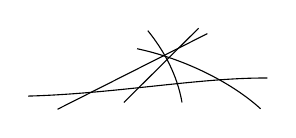
\begin{tikzpicture}[scale=.62]
\draw (0,.35) .. controls (1.8,.40) and (3.5,.73) .. (4.9,.72);
\draw (.6,.08) -- (3.67,1.63);
\draw (1.96,.22) -- (3.49,1.74);
\draw (2.45,1.69) .. controls (2.78,1.28) and (3.05,.79) .. (3.15,.22);
\draw (2.23,1.32) .. controls (3.13,1.13) and (4.12,.67) .. (4.76,.09);
\end{tikzpicture}}

\margin{$pq+2$ sommets\\ $N\geq5$}
$\mathrm{I}_{pq})$ Système formé de deux faisceaux de \inserted{$p$ et $q$} ps. droites concourantes $(p\geq q\geq2)$ plus \deleted{\unsure{leur|une}} ps. droite passant par les sommets de ces deux faisceaux $(p+q+1=N)$ (Cas de la ps. droite bigonale unique)
\figure{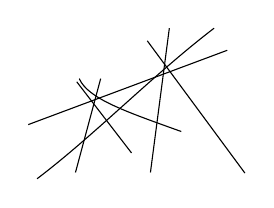
\begin{tikzpicture}[scale=.8]
\draw (.1,.92) -- (3.26,2.10);
\draw (.24,.06) .. controls (1.15,.75) and (2.07,1.70) .. (3.05,2.45);
\draw (.85,.16) -- (1.25,1.65);
\draw (.87,1.60) -- (1.74,.47);
\draw (.91,1.65) .. controls (1.05,1.33) and (1.64,1.13) .. (2.53,.81);
\draw (2.04,.16) -- (2.34,2.45);
\draw (1.99,2.25) -- (3.54,.15);
\end{tikzpicture}}

$2^\circ)$ Il n'existe pas de ps. droite bigonale \deleted{\unsure{de}}

\margin{$pq+2$ sommets\\ $N\geq5$}
$\deleted{\unsure{\mathrm I|\mathrm{II}}}\mathrm{II}_{pq})$ Système formé de deux faisceaux de $p$ et $q$ ps. droites concourantes $p\deleted{>}\geq q\geq2$, $p+q\deleted{\unsure{\geq}}=N\geq5$ (les deux faisceaux \unsure{incl.|i.e.} leurs sommets sont \deleted{\unsure{en pos}} alternés, \deleted{\unsure{le}} le cas ``minimal'' $p=\deleted{\unsure{3|2}}\unsure{2|3}$, $q=2$ est particulièrement intéressant\deleted{\unsure{)}}).
\figure{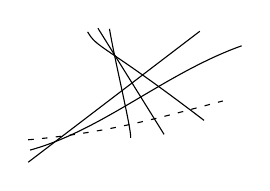
\begin{tikzpicture}[scale=.77]
\draw (0,.04) -- (2.83,2.20);
\draw (.03,.24) .. controls (1.23,.57) and (2.26,1.51) .. (3.52,1.96);
\draw[dash pattern=on 2pt off 3pt] (0,.41) .. controls (1.35,.53) and (2.14,.77) .. (3.21,1.05);
\draw (.98,2.19) .. controls (1.14,1.91) and (1.25,1.99) .. (2.90,.73);
\draw (1.15,2.25) -- (2.24,.50);
\draw (1.34,2.24) .. controls (1.43,1.70) and (1.70,.60) .. (1.69,.44);
\end{tikzpicture}}

\margin{$6$ sommets}
$\mathrm{II}_{4})$ \deleted{4 ps. droites en position} \inserted{Arrangement simple} de $4$ ps. droites

\margin{$10$ sommets}
$\mathrm{II}_{5})$ Arrangement simple de $5$ ps. droites.

\deleted{\unsure{Ds|Dans} le cas où il n'y a pas de ps. droite bigonale (i.e., pas $\mathrm{I}_{N}$, ni $\mathrm{I}_{p,q}$) \unsure{on est en}}
% archive sheet number: 22
